\documentclass[border=12pt]{standalone}
\def\pgfsysdriver{pgfsys-dvisvgm.def}
\usepackage[dvisvgm]{xcolor}
\usepackage{xeCJK}
\setCJKmainfont{HaranoAjiGothic-Regular.otf}[BoldFont=HaranoAjiGothic-Bold.otf]
\setCJKsansfont{HaranoAjiGothic-Regular.otf}[BoldFont=HaranoAjiGothic-Bold.otf]
\usepackage{amsmath,amssymb,tikz,lmodern}
\usetikzlibrary{arrows.meta,positioning,calc,fit,backgrounds}
\renewcommand{\familydefault}{\sfdefault}
\definecolor{ink}{HTML}{25322F}
\definecolor{green}{HTML}{246657}
\definecolor{tint}{HTML}{EEF4F0}
\definecolor{soft}{HTML}{C6D2CC}
\definecolor{muted}{HTML}{52615B}
\newif\ifJapanese
\newcommand{\Tx}[2]{\ifJapanese #1\else #2\fi}
\newcommand{\Eff}{\overline{\operatorname{Eff}}}
\newcommand{\heading}[3]{{\color{green}\bfseries #1\quad\Tx{#2}{#3}}\\[5pt]}
% A white rectangle makes the complete citation label clickable, including spaces.
\newcommand{\refurl}[2]{\special{dvisvgm:raw <a xlink:href="#1" target="_blank" rel="noopener noreferrer">}{\setlength{\fboxsep}{0pt}\colorbox{white}{\color{green}\underline{\strut #2}}}\special{dvisvgm:raw </a>}}
\tikzset{
 card/.style={draw=soft,fill=white,rounded corners=2pt,align=left,text=ink,font=\fontsize{10.5}{14}\selectfont,inner xsep=12pt,inner ysep=10pt,text width=14.4cm},
 half/.style={card,text width=6.45cm,minimum height=2.05cm},
 result/.style={card,draw=green,fill=tint,line width=.9pt},
 reason/.style={align=left,text=muted,font=\fontsize{9}{12}\selectfont,inner sep=0pt,text width=12.7cm},
 branchreason/.style={reason,text width=5.95cm},
 edge/.style={-{Stealth[length=2.4mm]},draw=green,line width=1pt},
 wire/.style={draw=green,line width=1pt},
}
% Keep the arrow in a dedicated left gutter; explanations never cover it.
\newcommand{\flow}[3]{
 \coordinate (#2-from) at ($(#1.south)+(-6.9,0)$);
 \coordinate (#2-to) at ($(#2.north)+(-6.9,0)$);
 \draw[edge] (#2-from)--(#2-to);
 \node[reason,anchor=west] (#2-reason) at ($(#2-from)!.5!(#2-to)+(.55,0)$) {#3};
}

\newcommand{\Cite}[2]{\refurl{#1}{#2}}

\Japanesefalse
\begin{document}
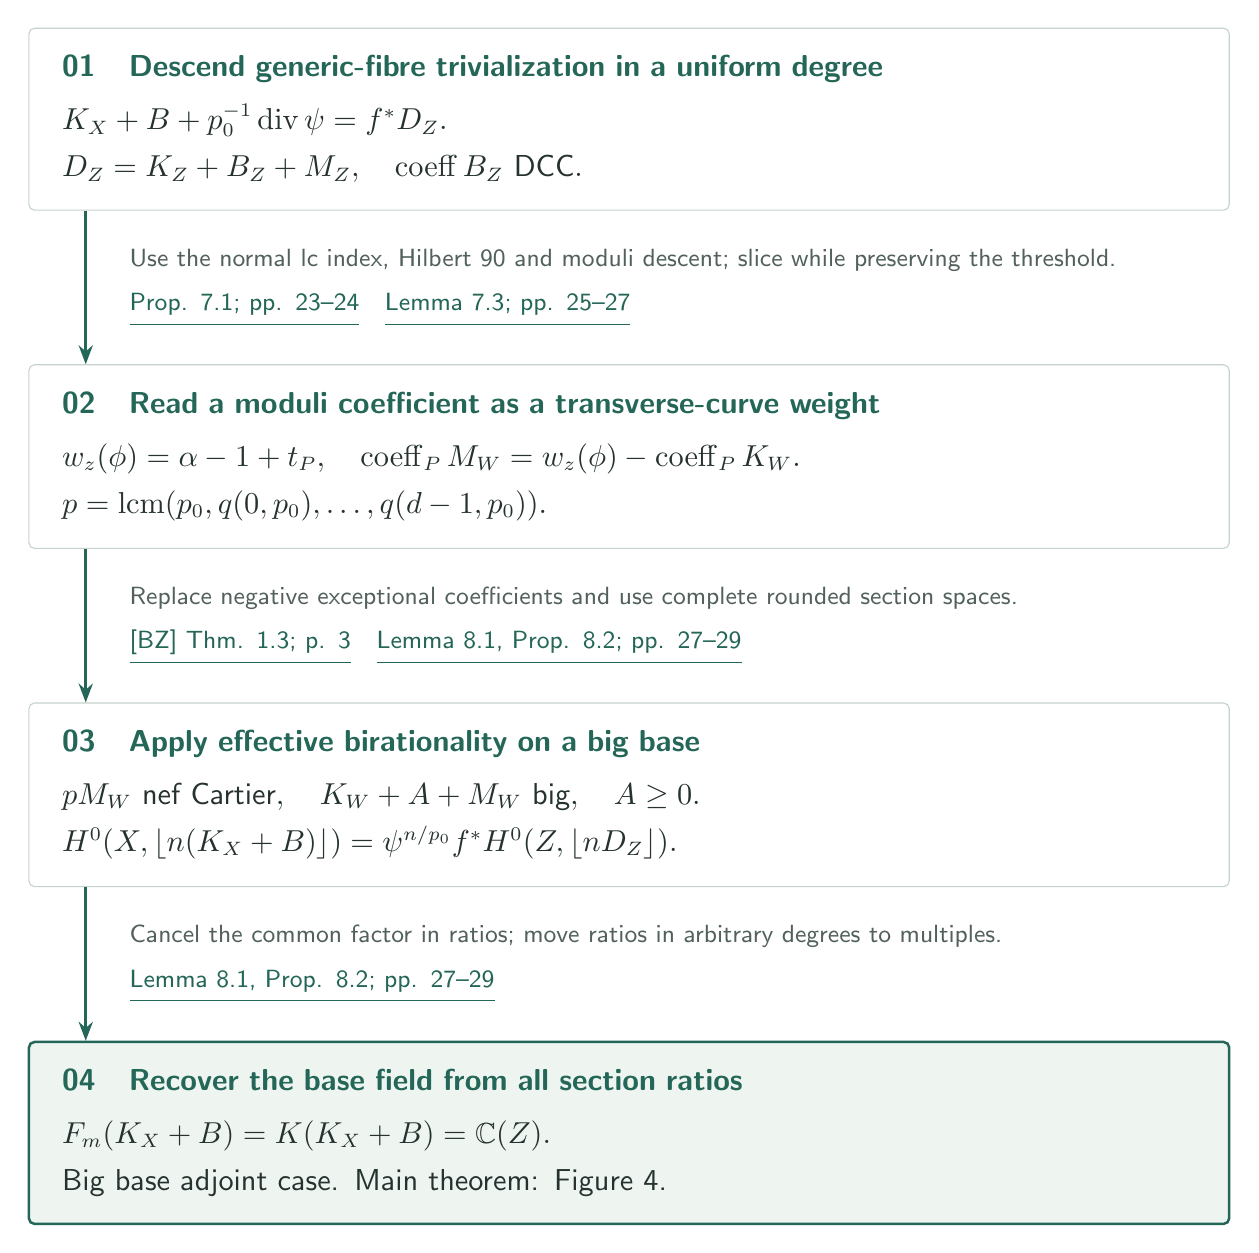
\begin{tikzpicture}
\node[card] (n0) {\heading{01}{一般ファイバーの自明化を一様な次数で降下}{Descend generic-fibre trivialization in a uniform degree}$K_X+B+p_0^{-1}\operatorname{div}\psi=f^*D_Z.$\\[3pt] $D_Z=K_Z+B_Z+M_Z,\quad \operatorname{coeff}B_Z\text{ DCC}.$};
\node[card,below=1.95cm of n0] (n1) {\heading{02}{横断曲線でmoduli係数を重みに置き換える}{Read a moduli coefficient as a transverse-curve weight}$w_z(\phi)=\alpha-1+t_P,\quad \operatorname{coeff}_P M_W=w_z(\phi)-\operatorname{coeff}_P K_W.$\\[3pt] $p=\operatorname{lcm}(p_0,q(0,p_0),\ldots,q(d-1,p_0)).$};
\flow{n0}{n1}{\Tx{normal lc指数・Hilbert 90・定性的moduli降下の後、閾値を保って切断。}{Use the normal lc index, Hilbert 90 and moduli descent; slice while preserving the threshold.}\\[4pt]\Cite{https://github.com/openai/math/blob/adc7f1241b42e322a6451854ab7e4b4c146bf78a/preprints/Uniform-log-Iitaka-fibrations-and-bounded-moduli-denominators-October-4-2026/uniform-log-iitaka.pdf}{Prop. 7.1; pp. 23--24}\quad \Cite{https://github.com/openai/math/blob/adc7f1241b42e322a6451854ab7e4b4c146bf78a/preprints/Uniform-log-Iitaka-fibrations-and-bounded-moduli-denominators-October-4-2026/uniform-log-iitaka.pdf}{Lemma 7.3; pp. 25--27}}
\node[card,below=1.95cm of n1] (n2) {\heading{03}{bigな底に有効双有理性を適用}{Apply effective birationality on a big base}$pM_W\text{ nef Cartier},\quad K_W+A+M_W\text{ big},\quad A\ge0.$\\[3pt] $H^0(X,\lfloor n(K_X+B)\rfloor)=\psi^{n/p_0}f^*H^0(Z,\lfloor nD_Z\rfloor).$};
\flow{n1}{n2}{\Tx{負の例外係数を被約例外境界に置換し、丸めた完全切断空間を使う。}{Replace negative exceptional coefficients and use complete rounded section spaces.}\\[4pt]\Cite{https://arxiv.org/pdf/1410.0938}{[BZ] Thm. 1.3; p. 3}\quad \Cite{https://github.com/openai/math/blob/adc7f1241b42e322a6451854ab7e4b4c146bf78a/preprints/Uniform-log-Iitaka-fibrations-and-bounded-moduli-denominators-October-4-2026/uniform-log-iitaka.pdf}{Lemma 8.1, Prop. 8.2; pp. 27--29}}
\node[result,below=1.95cm of n2] (n3) {\heading{04}{全切断比で底の体を回復する}{Recover the base field from all section ratios}$F_m(K_X+B)=K(K_X+B)=\mathbb C(Z).$\\[3pt] $\Tx{\text{底の随伴因子がbigの場合。主定理は第4図。}}{\text{Big base adjoint case. Main theorem: Figure 4.}}$};
\flow{n2}{n3}{\Tx{完全系の切断比から共通因子を消し、任意次数の比を倍数次数へ移す。}{Cancel the common factor in ratios; move ratios in arbitrary degrees to multiples.}\\[4pt]\Cite{https://github.com/openai/math/blob/adc7f1241b42e322a6451854ab7e4b4c146bf78a/preprints/Uniform-log-Iitaka-fibrations-and-bounded-moduli-denominators-October-4-2026/uniform-log-iitaka.pdf}{Lemma 8.1, Prop. 8.2; pp. 27--29}}
\end{tikzpicture}

\end{document}
